% Options for packages loaded elsewhere
\PassOptionsToPackage{unicode}{hyperref}
\PassOptionsToPackage{hyphens}{url}
%
\documentclass[
  ignorenonframetext,
  unknownkeysallowed]{beamer}
\usepackage{pgfpages}
\setbeamertemplate{caption}[numbered]
\setbeamertemplate{caption label separator}{: }
\setbeamercolor{caption name}{fg=normal text.fg}
\beamertemplatenavigationsymbolsempty
% Prevent slide breaks in the middle of a paragraph
\widowpenalties 1 10000
\raggedbottom
\setbeamertemplate{part page}{
  \centering
  \begin{beamercolorbox}[sep=16pt,center]{part title}
    \usebeamerfont{part title}\insertpart\par
  \end{beamercolorbox}
}
\setbeamertemplate{section page}{
  \centering
  \begin{beamercolorbox}[sep=12pt,center]{part title}
    \usebeamerfont{section title}\insertsection\par
  \end{beamercolorbox}
}
\setbeamertemplate{subsection page}{
  \centering
  \begin{beamercolorbox}[sep=8pt,center]{part title}
    \usebeamerfont{subsection title}\insertsubsection\par
  \end{beamercolorbox}
}
\AtBeginPart{
  \frame{\partpage}
}
\AtBeginSection{
  \ifbibliography
  \else
    \frame{\sectionpage}
  \fi
}
\AtBeginSubsection{
  \frame{\subsectionpage}
}
\usepackage{lmodern}
\usepackage{amssymb,amsmath}
\usepackage{ifxetex,ifluatex}
\ifnum 0\ifxetex 1\fi\ifluatex 1\fi=0 % if pdftex
  \usepackage[T1]{fontenc}
  \usepackage[utf8]{inputenc}
  \usepackage{textcomp} % provide euro and other symbols
\else % if luatex or xetex
  \usepackage{unicode-math}
  \defaultfontfeatures{Scale=MatchLowercase}
  \defaultfontfeatures[\rmfamily]{Ligatures=TeX,Scale=1}
\fi
\usecolortheme{beaver}
% Use upquote if available, for straight quotes in verbatim environments
\IfFileExists{upquote.sty}{\usepackage{upquote}}{}
\IfFileExists{microtype.sty}{% use microtype if available
  \usepackage[]{microtype}
  \UseMicrotypeSet[protrusion]{basicmath} % disable protrusion for tt fonts
}{}
\makeatletter
\@ifundefined{KOMAClassName}{% if non-KOMA class
  \IfFileExists{parskip.sty}{%
    \usepackage{parskip}
  }{% else
    \setlength{\parindent}{0pt}
    \setlength{\parskip}{6pt plus 2pt minus 1pt}}
}{% if KOMA class
  \KOMAoptions{parskip=half}}
\makeatother
\usepackage{xcolor}
\IfFileExists{xurl.sty}{\usepackage{xurl}}{} % add URL line breaks if available
\IfFileExists{bookmark.sty}{\usepackage{bookmark}}{\usepackage{hyperref}}
\hypersetup{
  pdftitle={COVID Monkeys},
  hidelinks,
  pdfcreator={LaTeX via pandoc}}
\urlstyle{same} % disable monospaced font for URLs
\newif\ifbibliography
\usepackage{graphicx,grffile}
\makeatletter
\def\maxwidth{\ifdim\Gin@nat@width>\linewidth\linewidth\else\Gin@nat@width\fi}
\def\maxheight{\ifdim\Gin@nat@height>\textheight\textheight\else\Gin@nat@height\fi}
\makeatother
% Scale images if necessary, so that they will not overflow the page
% margins by default, and it is still possible to overwrite the defaults
% using explicit options in \includegraphics[width, height, ...]{}
\setkeys{Gin}{width=\maxwidth,height=\maxheight,keepaspectratio}
% Set default figure placement to htbp
\makeatletter
\def\fps@figure{htbp}
\makeatother
\setlength{\emergencystretch}{3em} % prevent overfull lines
\providecommand{\tightlist}{%
  \setlength{\itemsep}{0pt}\setlength{\parskip}{0pt}}
\setcounter{secnumdepth}{-\maxdimen} % remove section numbering
\usepackage{dcolumn}
\usepackage{float}
\usepackage{graphicx}
\usepackage{booktabs}
\usepackage{longtable}
\usepackage{array}
\usepackage{multirow}
\usepackage{wrapfig}
\usepackage{colortbl}
\usepackage{pdflscape}
\usepackage{tabu}
\usepackage{threeparttable}
\usepackage{amsmath}
\makeatletter\beamer@ignorenonframefalse\makeatother
\makeatletter\def\fnum@table{\usebeamercolor{caption name}\usebeamerfont*{caption name}\tablename~\thetable}\makeatother
\usepackage[]{natbib}
\bibliographystyle{plainnat}

\title{COVID Monkeys}
\subtitle{HRV Analysis}
\author{}
\date{\vspace{-2.5em}September 13, 2020}

\begin{document}
\frame{\titlepage}

\begin{frame}{Introduction}
\protect\hypertarget{introduction}{}

\begin{itemize}
\tightlist
\item
  ECG analysis of monkeys with COVID
\item
  HRV performed of available signal
\item
  Monkeys all have SARS-CoV2 infection, half were treated with
  anti-inflammatories
\end{itemize}

\end{frame}

\begin{frame}{Quality of Signal Processing Efforts}
\protect\hypertarget{quality-of-signal-processing-efforts}{}

\begin{table}

\caption{\label{tab:unnamed-chunk-1}Best quality per session/lead}
\centering
\fontsize{6}{8}\selectfont
\begin{tabular}[t]{rlrlrr}
\toprule
session & names & visit & lead & tot\_wind & percent\_not\_analyzed\\
\midrule
\cellcolor{gray!6}{1} & \cellcolor{gray!6}{rat11} & \cellcolor{gray!6}{1} & \cellcolor{gray!6}{LII} & \cellcolor{gray!6}{58} & \cellcolor{gray!6}{0.0}\\
2 & 06\_112 & 1 & NA & NA & NA\\
\cellcolor{gray!6}{3} & \cellcolor{gray!6}{rat11} & \cellcolor{gray!6}{2} & \cellcolor{gray!6}{LII} & \cellcolor{gray!6}{58} & \cellcolor{gray!6}{19.0}\\
4 & 06\_112 & 2 & LII & 52 & 71.2\\
\cellcolor{gray!6}{5} & \cellcolor{gray!6}{rat11} & \cellcolor{gray!6}{3} & \cellcolor{gray!6}{LII} & \cellcolor{gray!6}{58} & \cellcolor{gray!6}{27.6}\\
\addlinespace
6 & 06\_112 & 3 & LII & 58 & 48.3\\
\cellcolor{gray!6}{7} & \cellcolor{gray!6}{06\_112} & \cellcolor{gray!6}{4} & \cellcolor{gray!6}{aVF} & \cellcolor{gray!6}{30} & \cellcolor{gray!6}{0.0}\\
8 & rat11 & 4 & LI & 70 & 24.3\\
\cellcolor{gray!6}{9} & \cellcolor{gray!6}{5\_215} & \cellcolor{gray!6}{1} & \cellcolor{gray!6}{aVF} & \cellcolor{gray!6}{18} & \cellcolor{gray!6}{0.0}\\
10 & rqv9 & 1 & aVF & 54 & 0.0\\
\addlinespace
\cellcolor{gray!6}{11} & \cellcolor{gray!6}{rlf10} & \cellcolor{gray!6}{1} & \cellcolor{gray!6}{aVF} & \cellcolor{gray!6}{37} & \cellcolor{gray!6}{2.7}\\
12 & 06\_112 & 5 & aVF & 127 & 0.0\\
\cellcolor{gray!6}{13} & \cellcolor{gray!6}{rat11} & \cellcolor{gray!6}{5} & \cellcolor{gray!6}{aVF} & \cellcolor{gray!6}{135} & \cellcolor{gray!6}{0.0}\\
14 & 5\_215 & 2 & aVL & 72 & 0.0\\
\cellcolor{gray!6}{15} & \cellcolor{gray!6}{rqv9} & \cellcolor{gray!6}{2} & \cellcolor{gray!6}{aVF} & \cellcolor{gray!6}{57} & \cellcolor{gray!6}{0.0}\\
\addlinespace
16 & rlf10 & 2 & aVF & 121 & 0.0\\
\cellcolor{gray!6}{17} & \cellcolor{gray!6}{rlf10} & \cellcolor{gray!6}{3} & \cellcolor{gray!6}{aVF} & \cellcolor{gray!6}{73} & \cellcolor{gray!6}{0.0}\\
18 & rqv9 & 3 & aVF & 42 & 0.0\\
\cellcolor{gray!6}{19} & \cellcolor{gray!6}{rqv9} & \cellcolor{gray!6}{4} & \cellcolor{gray!6}{aVF} & \cellcolor{gray!6}{75} & \cellcolor{gray!6}{0.0}\\
20 & 5\_215 & 3 & aVF & 25 & 0.0\\
\addlinespace
\cellcolor{gray!6}{21} & \cellcolor{gray!6}{5\_215} & \cellcolor{gray!6}{4} & \cellcolor{gray!6}{Vx} & \cellcolor{gray!6}{54} & \cellcolor{gray!6}{0.0}\\
22 & rlf10 & 4 & LIII & 103 & 32.0\\
\bottomrule
\end{tabular}
\end{table}

\end{frame}

\begin{frame}{HRV Findings}
\protect\hypertarget{hrv-findings}{}

\begin{table}[H]
\centering\begingroup\fontsize{6}{8}\selectfont

\begin{tabular}{rrrrrrrr}
\toprule
session & NN & SDNN & RMSSD & PNN50 & HF & LF & APEN\\
\midrule
\cellcolor{gray!6}{1} & \cellcolor{gray!6}{341} & \cellcolor{gray!6}{13.06} & \cellcolor{gray!6}{4.96} & \cellcolor{gray!6}{0.000} & \cellcolor{gray!6}{59.17} & \cellcolor{gray!6}{249.83} & \cellcolor{gray!6}{0.575}\\
3 & 323 & 11.75 & 15.89 & 3.951 & 45.58 & 59.66 & 0.744\\
\cellcolor{gray!6}{4} & \cellcolor{gray!6}{326} & \cellcolor{gray!6}{19.95} & \cellcolor{gray!6}{31.74} & \cellcolor{gray!6}{15.081} & \cellcolor{gray!6}{59.62} & \cellcolor{gray!6}{54.85} & \cellcolor{gray!6}{0.665}\\
5 & 349 & 8.25 & 9.50 & 1.266 & 22.37 & 24.90 & 0.720\\
\cellcolor{gray!6}{6} & \cellcolor{gray!6}{342} & \cellcolor{gray!6}{16.82} & \cellcolor{gray!6}{25.47} & \cellcolor{gray!6}{8.304} & \cellcolor{gray!6}{73.46} & \cellcolor{gray!6}{48.28} & \cellcolor{gray!6}{0.567}\\
\addlinespace
7 & 370 & 8.91 & 6.88 & 0.243 & 17.30 & 26.60 & 1.117\\
\cellcolor{gray!6}{8} & \cellcolor{gray!6}{430} & \cellcolor{gray!6}{7.25} & \cellcolor{gray!6}{6.24} & \cellcolor{gray!6}{0.208} & \cellcolor{gray!6}{9.60} & \cellcolor{gray!6}{30.01} & \cellcolor{gray!6}{1.028}\\
9 & 402 & 22.85 & 11.99 & 0.938 & 190.18 & 252.91 & 0.637\\
\cellcolor{gray!6}{10} & \cellcolor{gray!6}{449} & \cellcolor{gray!6}{12.77} & \cellcolor{gray!6}{10.18} & \cellcolor{gray!6}{1.546} & \cellcolor{gray!6}{53.81} & \cellcolor{gray!6}{35.00} & \cellcolor{gray!6}{0.918}\\
11 & 435 & 11.75 & 17.69 & 3.841 & 26.56 & 9.63 & 0.991\\
\addlinespace
\cellcolor{gray!6}{12} & \cellcolor{gray!6}{323} & \cellcolor{gray!6}{5.83} & \cellcolor{gray!6}{6.43} & \cellcolor{gray!6}{0.075} & \cellcolor{gray!6}{13.36} & \cellcolor{gray!6}{12.36} & \cellcolor{gray!6}{1.142}\\
13 & 430 & 22.52 & 15.15 & 5.486 & 77.02 & 276.56 & 0.787\\
\cellcolor{gray!6}{14} & \cellcolor{gray!6}{339} & \cellcolor{gray!6}{9.61} & \cellcolor{gray!6}{8.77} & \cellcolor{gray!6}{0.477} & \cellcolor{gray!6}{20.89} & \cellcolor{gray!6}{39.87} & \cellcolor{gray!6}{1.079}\\
15 & 440 & 22.76 & 12.55 & 1.094 & 24.47 & 108.38 & 0.814\\
\cellcolor{gray!6}{16} & \cellcolor{gray!6}{434} & \cellcolor{gray!6}{7.94} & \cellcolor{gray!6}{6.28} & \cellcolor{gray!6}{0.285} & \cellcolor{gray!6}{4.25} & \cellcolor{gray!6}{10.21} & \cellcolor{gray!6}{0.930}\\
\addlinespace
17 & 485 & 11.86 & 6.07 & 0.079 & 9.21 & 36.98 & 0.919\\
\cellcolor{gray!6}{18} & \cellcolor{gray!6}{444} & \cellcolor{gray!6}{10.17} & \cellcolor{gray!6}{8.28} & \cellcolor{gray!6}{0.323} & \cellcolor{gray!6}{40.60} & \cellcolor{gray!6}{49.93} & \cellcolor{gray!6}{0.981}\\
19 & 474 & 27.42 & 17.03 & 3.251 & 68.92 & 289.17 & 0.712\\
\cellcolor{gray!6}{20} & \cellcolor{gray!6}{322} & \cellcolor{gray!6}{7.98} & \cellcolor{gray!6}{6.92} & \cellcolor{gray!6}{0.307} & \cellcolor{gray!6}{34.85} & \cellcolor{gray!6}{64.39} & \cellcolor{gray!6}{1.114}\\
21 & 340 & 14.66 & 9.51 & 0.710 & 74.40 & 219.41 & 0.989\\
\addlinespace
\cellcolor{gray!6}{22} & \cellcolor{gray!6}{425} & \cellcolor{gray!6}{16.02} & \cellcolor{gray!6}{11.39} & \cellcolor{gray!6}{2.084} & \cellcolor{gray!6}{31.75} & \cellcolor{gray!6}{52.75} & \cellcolor{gray!6}{0.897}\\
\bottomrule
\end{tabular}
\endgroup{}
\end{table}

\end{frame}

\begin{frame}{Summary Longitudinal HRV}
\protect\hypertarget{summary-longitudinal-hrv}{}

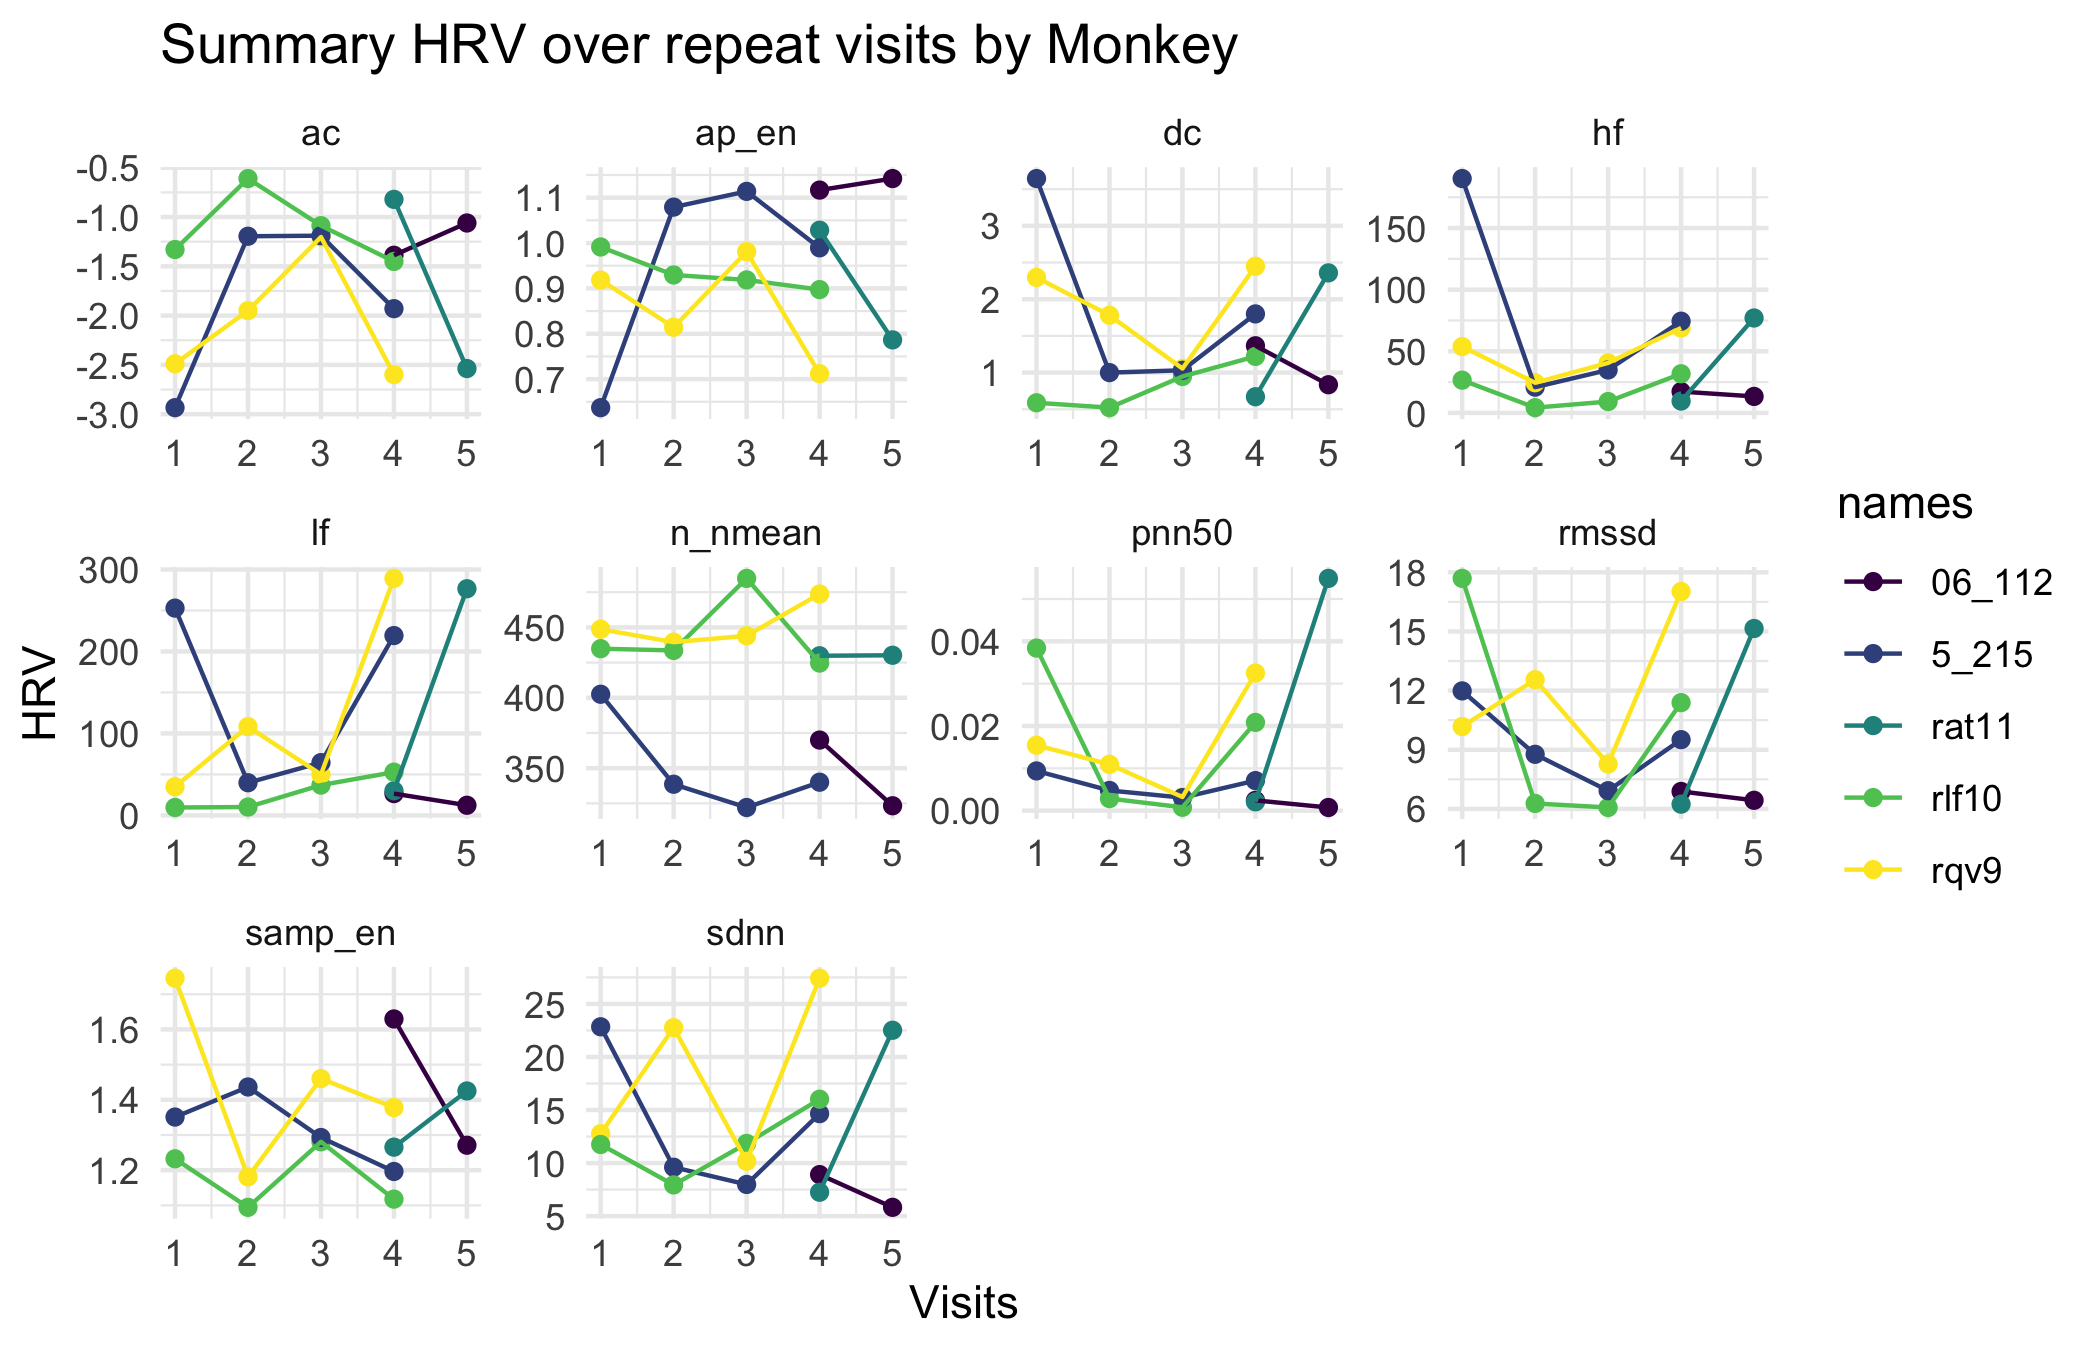
\includegraphics{/Users/asshah4/Box Sync/projects/covid-monkeys/products/draft-findings_files/figure-beamer/unnamed-chunk-3-1.png}

\end{frame}

\begin{frame}{Summary Longitudinal HRV by Treatment}
\protect\hypertarget{summary-longitudinal-hrv-by-treatment}{}

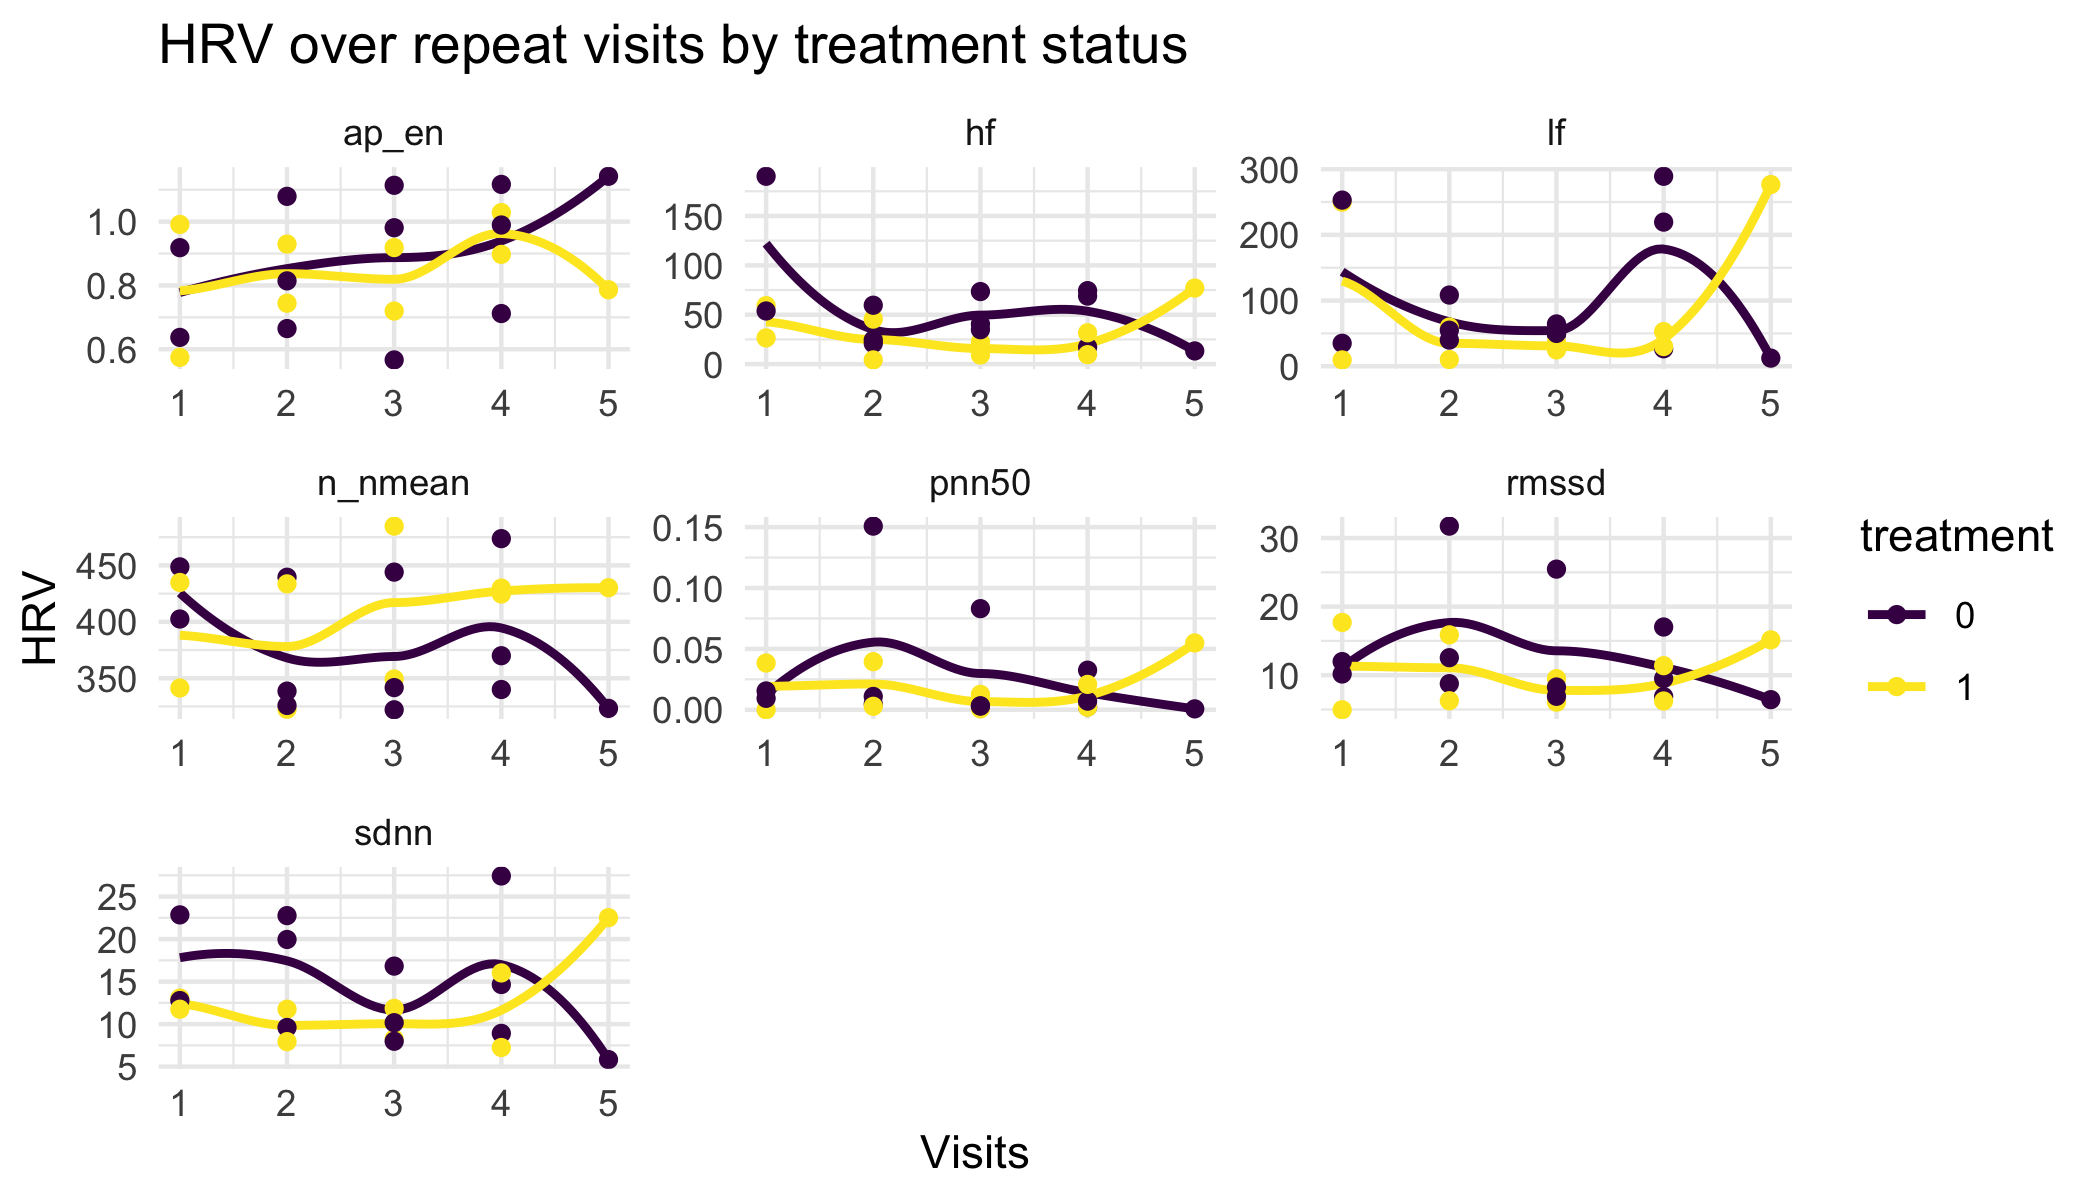
\includegraphics{/Users/asshah4/Box Sync/projects/covid-monkeys/products/draft-findings_files/figure-beamer/unnamed-chunk-4-1.png}

\end{frame}

\begin{frame}{Summary by Treatment}
\protect\hypertarget{summary-by-treatment}{}

\captionsetup[table]{labelformat=empty,skip=1pt}
\begin{longtable}{lrrrrrrr}
\caption*{
\large HRV Changes by Treatment Groups\\ 
\small Measured at Repeat Visits\\ 
} \\ 
\toprule
& \multicolumn{7}{c}{HRV Measurements} \\ 
 \cmidrule(lr){2-8}
Treated & n\_nmean & sdnn & rmssd & pnn50 & hf & lf & ap\_en \\ 
\midrule
\multicolumn{1}{l}{0} \\ 
\midrule
1 & $425.6$ & $17.8$ & $11.1$ & $0.0$ & $122.0$ & $144.0$ & $0.8$ \\ 
2 & $368.0$ & $17.4$ & $17.7$ & $0.1$ & $35.0$ & $67.7$ & $0.9$ \\ 
3 & $369.3$ & $11.7$ & $13.6$ & $0.0$ & $49.6$ & $54.2$ & $0.9$ \\ 
4 & $394.6$ & $17.0$ & $11.1$ & $0.0$ & $53.5$ & $178.4$ & $0.9$ \\ 
5 & $323.3$ & $5.8$ & $6.4$ & $0.0$ & $13.4$ & $12.4$ & $1.1$ \\ 
\midrule
\multicolumn{1}{l}{1} \\ 
\midrule
1 & $388.1$ & $12.4$ & $11.3$ & $0.0$ & $42.9$ & $129.7$ & $0.8$ \\ 
2 & $378.1$ & $9.8$ & $11.1$ & $0.0$ & $24.9$ & $34.9$ & $0.8$ \\ 
3 & $417.1$ & $10.1$ & $7.8$ & $0.0$ & $15.8$ & $30.9$ & $0.8$ \\ 
4 & $427.3$ & $11.6$ & $8.8$ & $0.0$ & $20.7$ & $41.4$ & $1.0$ \\ 
5 & $430.2$ & $22.5$ & $15.2$ & $0.1$ & $77.0$ & $276.6$ & $0.8$ \\ 
\bottomrule
\end{longtable}

\end{frame}

\begin{frame}{Repeat Measures Analysis}
\protect\hypertarget{repeat-measures-analysis}{}

\begin{table}[H]
\centering\begingroup\fontsize{6}{8}\selectfont

\begin{tabular}{lllrrrrr}
\toprule
hrv & stratum & term & df & sumsq & meansq & statistic & p.value\\
\midrule
\cellcolor{gray!6}{n\_nmean} & \cellcolor{gray!6}{names} & \cellcolor{gray!6}{visit} & \cellcolor{gray!6}{1} & \cellcolor{gray!6}{1.89e+04} & \cellcolor{gray!6}{1.89e+04} & \cellcolor{gray!6}{2.235} & \cellcolor{gray!6}{0.232}\\
n\_nmean & Within & visit & 1 & 1.97e+03 & 1.97e+03 & 1.773 & 0.203\\
\cellcolor{gray!6}{sdnn} & \cellcolor{gray!6}{names} & \cellcolor{gray!6}{visit} & \cellcolor{gray!6}{1} & \cellcolor{gray!6}{1.46e+01} & \cellcolor{gray!6}{1.46e+01} & \cellcolor{gray!6}{0.479} & \cellcolor{gray!6}{0.539}\\
sdnn & Within & visit & 1 & 2.00e-03 & 2.00e-03 & 0.000 & 0.995\\
\cellcolor{gray!6}{rmssd} & \cellcolor{gray!6}{names} & \cellcolor{gray!6}{visit} & \cellcolor{gray!6}{1} & \cellcolor{gray!6}{1.16e+02} & \cellcolor{gray!6}{1.16e+02} & \cellcolor{gray!6}{5.378} & \cellcolor{gray!6}{0.103}\\
\addlinespace
rmssd & Within & visit & 1 & 6.04e+01 & 6.04e+01 & 1.318 & 0.269\\
\cellcolor{gray!6}{pnn50} & \cellcolor{gray!6}{names} & \cellcolor{gray!6}{visit} & \cellcolor{gray!6}{1} & \cellcolor{gray!6}{6.00e-03} & \cellcolor{gray!6}{6.00e-03} & \cellcolor{gray!6}{18.872} & \cellcolor{gray!6}{0.023}\\
pnn50 & Within & visit & 1 & 1.00e-03 & 1.00e-03 & 1.145 & 0.301\\
\cellcolor{gray!6}{hf} & \cellcolor{gray!6}{names} & \cellcolor{gray!6}{visit} & \cellcolor{gray!6}{1} & \cellcolor{gray!6}{2.04e+02} & \cellcolor{gray!6}{2.04e+02} & \cellcolor{gray!6}{0.079} & \cellcolor{gray!6}{0.797}\\
hf & Within & visit & 1 & 1.66e+03 & 1.66e+03 & 1.070 & 0.317\\
\addlinespace
\cellcolor{gray!6}{lf} & \cellcolor{gray!6}{names} & \cellcolor{gray!6}{visit} & \cellcolor{gray!6}{1} & \cellcolor{gray!6}{6.18e+03} & \cellcolor{gray!6}{6.18e+03} & \cellcolor{gray!6}{0.422} & \cellcolor{gray!6}{0.562}\\
lf & Within & visit & 1 & 3.88e+03 & 3.88e+03 & 0.428 & 0.523\\
\cellcolor{gray!6}{ap\_en} & \cellcolor{gray!6}{names} & \cellcolor{gray!6}{visit} & \cellcolor{gray!6}{1} & \cellcolor{gray!6}{2.00e-02} & \cellcolor{gray!6}{2.00e-02} & \cellcolor{gray!6}{0.804} & \cellcolor{gray!6}{0.436}\\
ap\_en & Within & visit & 1 & 1.17e-01 & 1.17e-01 & 3.890 & 0.067\\
\bottomrule
\end{tabular}
\endgroup{}
\end{table}

\end{frame}

\end{document}
